% Compile from this directory with: tectonic ieee-report.tex
% This source is self-contained: diagrams and references are embedded.
\documentclass[conference,a4paper]{IEEEtran}
\usepackage[T1]{fontenc}
\usepackage{amsmath,amssymb}
\usepackage{booktabs,array}
\usepackage{graphicx}
\usepackage{tikz}
\usetikzlibrary{arrows.meta,positioning}
\usepackage{cite}
\usepackage{etoolbox}
% Keep IEEE layout while using hyphens in the abstract and keyword labels.
\patchcmd{\abstract}{---}{ - }{}{}
\patchcmd{\IEEEkeywords}{---}{ - }{}{}
\usepackage[hidelinks]{hyperref}
\usepackage{url}
\Urlmuskip=0mu plus 1mu
\makeatletter
\g@addto@macro\UrlBreaks{\do\a\do\b\do\c\do\d\do\e\do\f\do\0\do\1\do\2\do\3\do\4\do\5\do\6\do\7\do\8\do\9}
\makeatother
\urlstyle{same}
\newcommand{\GF}{Good Fit}
\newcommand{\PF}{Potential Fit}
\newcommand{\NF}{No Fit}
\newcommand{\artifact}[1]{\texttt{\detokenize{#1}}}
\hypersetup{pdftitle={Resume-Job Matching with Compact Transformers: Development, Evaluation, and Deployment},pdfauthor={Pottabathini Vivekananda, Vikas Eranki, Manasa, Bhavani Shanker}}

\title{Resume-Job Matching with Compact Transformers:\\Development, Evaluation, and Deployment}
\author{\IEEEauthorblockN{Pottabathini Vivekananda, Vikas Eranki, Manasa, and Bhavani Shanker}
\IEEEauthorblockA{Newton School of Technology, Rishihood University\\Sonipat, India}}
\begin{document}
\maketitle

\begin{abstract}
Comparing resumes with job descriptions requires evaluating relevant experience while handling noisy documents, class imbalance, and limited model context. This report presents an end-to-end, three-class resume-job matching prototype with lexical baselines, fine-tuned MiniLM and DistilBERT classifiers, and a deployed Streamlit interface. Experiments use a public dataset of 8,000 labelled pairs. Conflicting and duplicate training records are removed, and job-grouped validation separates job descriptions across training, validation, and the official test set. A section-aware input experiment and class-weighted training are evaluated against the original DistilBERT. Class weighting increases validation macro-F1 from 0.3540 to 0.3582, leading to a selection recorded before test evaluation. On the official test set, the selected model achieves macro-F1 0.3563, while the fixed TF-IDF comparator achieves 0.4058. Error review and robustness tests expose weak suitable-candidate recall and sensitivity to document order and long prefixes. The interface accepts text or PDFs, uses local English OCR for scans, and reports truncation. The contribution is a reproducible engineering workflow and measured prototype, with explicit limits on model reliability and business readiness.
\end{abstract}
\begin{IEEEkeywords}
resume-job matching, natural language processing, DistilBERT, MiniLM, class imbalance, OCR, model deployment
\end{IEEEkeywords}

\section{Introduction}
Recruiters compare a candidate's qualifications, projects, and experience with requirements spread across a job description. The same skill can be expressed in different ways, while shared vocabulary can conceal differences in seniority, domain experience, or mandatory qualifications. These properties make resume-job matching an NLP problem whose usefulness must be assessed beyond a few favourable examples.

The project frames matching as supervised classification of a resume-job pair into \GF, \PF, or \NF. The intended user is a recruiter or hiring manager who reviews the suggestion. The prototype supports one pair per interaction; it does not implement automatic rejection, recruitment decisions, or batch applicant ranking. Its evaluation concerns a largely known candidate pool paired with unseen jobs, because resumes overlap across the available splits.

The work follows an industry-oriented development process: define the problem, audit data, establish lexical references, train compact transformer candidates, evaluate improvement attempts, and deploy a guarded application. Existing model training is preserved as the evidence for the classifier used by the application. No generative matching API, external reasoning service, or claim of newly trained OCR is part of the delivered system.

The main contributions are: (1) a repeatable dataset audit and job-grouped split protocol; (2) matched MiniLM and DistilBERT development with explicit token-coverage reporting; (3) documented section-selection and class-weighting iterations, paired error review, and robustness testing; and (4) a CPU deployment with PDF/OCR inputs, safe failures, and scoped performance measurements. The results do not establish transformer superiority or readiness for real hiring.

\section{Related Work}
Maheshwary and Misra study resume-job matching using a deep Siamese network \cite{siamese}. Lavi \emph{et al.}\ introduce conSultantBERT, a fine-tuned Siamese sentence-embedding approach to matching heterogeneous resume and vacancy text \cite{consultant}. ConFit combines augmentation and contrastive learning \cite{confit}; ConFit v2 investigates hypothetical resume embeddings and hard negatives \cite{confit2}. These works informed the comparison of lexical and learned representations, but their ranking, binary matching, and data-access settings differ from this project's three-class task. Their reported scores are not treated as directly comparable benchmarks.

The calibrated matching study \cite{calibrated} supplied a practical reference for TF-IDF methods on an accessible three-class dataset. The project reproduces reference methods rather than claiming an exact reproduction of its full hybrid system, calibration, or selective refusal. DistilBERT \cite{distilbert} and MiniLM \cite{minilm} provide pretrained compact transformer encoders that can be fine-tuned within the recorded Colab resources. Their general NLP capabilities motivate testing, but do not guarantee that fine-tuning will learn dependable recruitment reasoning.

\section{Data Understanding and Preparation}
\subsection{Dataset and Quality Audit}
The source dataset, \nolinkurl{cnamuangtoun/resume-job-description-fit} \cite{dataset}, contains resume text, job-description text, and a three-class label. The recorded revision is stored in the split manifest. Its original training split has 6,241 pairs and its official test split has 1,759 pairs. Across all 8,000 records, the class counts are 2,000 \GF, 2,000 \PF, and 4,000 \NF. The initial audit finds no missing or empty required fields.

Six training pair groups contain conflicting labels. Removing all 12 associated rows and one extra same-label duplicate leaves 6,228 training-pool rows. The original official-test records are retained. Pair duplication is also checked after preparation, since normalization can make distinct raw strings equivalent. Public access does not establish the dataset's collection method, consent, or reuse licence; these remain unresolved in the project documentation. The labels are treated as supplied annotations, not verified hiring outcomes.

\subsection{Text Preparation}
Transformer preparation applies Unicode NFKC normalization, retains visible Markdown link text, replaces email addresses, URLs, and qualifying phone patterns with placeholders, and normalizes whitespace. It preserves case, line breaks, and technical punctuation. This reduces formatting noise and some contact information; names, employers, educational institutions, and other identifiers can remain. It is therefore not complete anonymization.

TF-IDF retains the historical baseline cleaning, including lowercasing and its original character handling. The reference uses full cleaned documents, whereas transformer pairs are shortened to their context limit. The evaluation consequently compares complete approaches, not an isolated architecture change with identical information exposure.

\subsection{Job-Grouped Validation}
The historical baseline notebook uses a label-stratified pair split. Later experiments instead group normalized job descriptions using stable identifiers and use the first fold of \texttt{StratifiedGroupKFold} with five folds, shuffling, and seed 42. This creates one held-out validation split, not five trained cross-validation models. Table~\ref{tab:splits} lists the resulting shared protocol.

\begin{table}[t]
\caption{Shared M3 Split Counts}
\label{tab:splits}
\centering\footnotesize
\begin{tabular}{lrrrrr}
\toprule
Split & \GF & \PF & \NF & Total & Jobs\\
\midrule
Training & 1,258 & 1,223 & 2,600 & 5,081 & 229\\
Validation & 280 & 331 & 536 & 1,147 & 51\\
Official test & 458 & 444 & 857 & 1,759 & 71\\
\bottomrule
\end{tabular}
\end{table}

No prepared job or complete pair is shared across splits. However, 429 unique resumes are shared between training and validation, 473 between training and test, and 357 between validation and test. These are documented evaluation boundaries rather than a claim of fully independent applicants. Saved source-row identifiers, dataset revision, counts, and overlap reports allow exact reconstruction of the selected rows.

\section{Model Development}
\subsection{Lexical References}
The historical notebook implements TF-IDF cosine similarity and paired TF-IDF with stochastic gradient descent (SGD). Cosine thresholds are selected on validation data. Its saved test macro-F1 values are 0.3708 and 0.4100, respectively. These historical results use the earlier split protocol and are not substituted into the later shared-split comparison.

For the shared protocol, paired TF-IDF concatenates the cleaned resume and job description with explicit document markers. The vectorizer uses word unigrams and bigrams, at most 50,000 features, minimum document frequency 3, maximum document frequency 0.98, English stop words, and sublinear term frequency. It is fitted only on training text. An L2-regularized SGD classifier uses logistic loss, $\alpha=10^{-5}$, and seed 42. The recorded vocabulary has 50,000 features; fitting the vectorizer takes 16.63~s and the classifier 6.66~s in the saved CPU run.

\subsection{Fine-Tuned Compact Transformers}
The candidates are \nolinkurl{microsoft/MiniLM-L12-H384-uncased} and \nolinkurl{distilbert/distilbert-base-uncased}. Each receives a three-class classification head and is fine-tuned end to end. The recorded parameter counts are 33,361,155 for MiniLM and 66,955,779 for DistilBERT, including the task heads.

The input order is resume followed by job description. Each pair includes three special tokens and has a maximum length of 512 tokens. Right-side \texttt{longest\_first} truncation removes tokens from the longer component as necessary. MiniLM receives token-type IDs; DistilBERT does not. A dynamic collator pads batches to a multiple of eight.

The coverage audit is important: 99.63\% of training pairs and 99.39\% of validation pairs exceed 512 tokens. Mean retained token coverage is 34.76\% and 37.84\%, respectively. These are averages of per-pair retention values, not ratios of aggregate mean lengths. The input policy cannot process every supplied word, even when a document passes the application's character limit.

\begin{table}[t]
\caption{Shared Transformer Training Settings}
\label{tab:training}
\centering\footnotesize
\begin{tabular}{ll}
\toprule
Setting & Recorded value\\
\midrule
Maximum epochs & 3\\
Training/evaluation batch size & 8 / 16\\
Gradient accumulation & 2 steps\\
Effective training batch size & 16\\
Optimizer & AdamW\\
Learning rate / weight decay & $2\times10^{-5}$ / 0.01\\
Schedule / warmup & Linear / 96 updates\\
Gradient clipping & Norm 1.0\\
Seed & 42\\
Precision and accelerator & FP16, one Tesla T4\\
Checkpoint metric & Validation macro-F1\\
Evaluation / saving & Each epoch\\
Early-stopping patience & 1 epoch\\
\bottomrule
\end{tabular}
\end{table}

The runs use the shared settings in Table~\ref{tab:training}, with 318 optimizer updates per epoch and 954 over three completed epochs. Selected checkpoints occur at epoch two. Saved-model checks compare state tensors, tokenizer configuration, label mappings, and aligned-precision inference. These verify export integrity, not task accuracy or generalization.

\subsection{Section-Aware Input Experiment}
The first DistilBERT iteration detects headings such as skills, experience, education, requirements, and responsibilities. The fixed initial content budgets are 304 resume tokens and 205 job tokens, leaving three special tokens. Within-document quotas prioritize sections, and unused space can be reassigned within the 512-token pair limit. Unrecognized text remains in the current section or preamble.

Training and validation inputs are built using this policy, while the official test set is not processed for this experiment. The input policy is fixed before training or validation-based selection. This run retains the unweighted loss and original training arguments. Its purpose is to test whether prioritizing sections improves the limited-context representation, not to assume that section headings establish qualification evidence.

\subsection{Class-Weighted Training}
The second iteration restores the original \texttt{longest\_first} input policy and changes the training loss. Only training counts determine class weights:
\begin{equation}
w_c=\frac{N}{C n_c},\qquad C=3,
\end{equation}
where $N$ is the number of training rows and $n_c$ is the count for class $c$. The weights for \GF, \PF, and \NF\ are 1.3463, 1.3848, and 0.6514. For a batch $B$, the weighted mean cross-entropy is
\begin{equation}
\mathcal{L}_{B}=-\frac{\sum_{i\in B} w_{y_i}\log p_\theta(y_i\mid r_i,j_i)}{\sum_{i\in B} w_{y_i}}.
\end{equation}
The custom training loss is manually checked before optimization. The model starts from the pretrained checkpoint rather than continuing the section-aware run. Apart from the loss and output directory, the recorded training configuration matches the original DistilBERT experiment.

\section{Evaluation Protocol and Results}
\subsection{Metrics and Selection}
Macro-F1 is the primary metric because each class contributes equally:
\begin{equation}
F_{1,c}=\frac{2P_cR_c}{P_c+R_c},\qquad
F_{1,\mathrm{macro}}=\frac{1}{3}\sum_{c=1}^{3}F_{1,c}.
\end{equation}
Undefined class precision or F1 is handled as zero in the recorded reports. Accuracy, weighted F1, class recall, and confusion matrices provide supporting views. No calibrated probability or percentage match is exposed by the application.

Five candidates are compared using validation evidence. Before official-test inference, the project records weighted DistilBERT as selected and original DistilBERT and TF-IDF as fixed comparators. The selection file includes the weight hash, input policy, and decision timestamp. No test-driven threshold tuning or reselection follows. MiniLM and the section-aware model are not evaluated on the official test in this final comparison.

\begin{table}[t]
\caption{Validation Results on Shared Rows}
\label{tab:validation}
\centering\footnotesize
\setlength{\tabcolsep}{4pt}
\begin{tabular}{lrrr}
\toprule
Model & Macro-F1 & Accuracy & \PF\ recall\\
\midrule
TF-IDF + SGD & 0.2923 & 0.4429 & 0.1964\\
MiniLM & 0.3081 & 0.4682 & 0.0000\\
DistilBERT & 0.3540 & 0.4752 & 0.1088\\
Section-aware DistilBERT & 0.3258 & 0.4786 & 0.1813\\
Weighted DistilBERT & \textbf{0.3582} & 0.4673 & 0.1662\\
\bottomrule
\end{tabular}
\end{table}

\subsection{Validation Comparison}
Table~\ref{tab:validation} shows a 0.0459 macro-F1 increase from MiniLM to original DistilBERT for these runs. MiniLM predicts no validation examples as \PF. Section-aware inputs reduce macro-F1 by 0.0282 relative to original DistilBERT, despite raising \PF\ recall. Its \GF\ recall falls from 0.2107 to 0.0500.

Class weighting produces a smaller 0.0042 macro-F1 increase. Its validation \GF\ recall falls to 0.1679, and accuracy also decreases. The weighted model fixes 59 original validation errors but introduces 68 regressions: 12 fixes and 24 regressions for \GF, 31 and 12 for \PF, and 16 and 32 for \NF. Macro-F1 can improve despite fewer correct predictions because it weighs per-class F1 equally. No repeated-seed study or significance test establishes that this small gain is reliable.

\begin{table*}[t]
\caption{Official-Test Results for the Preselected Model and Fixed Comparators}
\label{tab:test}
\centering\small
\begin{tabular}{llrrrrr}
\toprule
Model & Role & Macro-F1 & Accuracy & \GF\ recall & \PF\ recall & \NF\ recall\\
\midrule
Weighted DistilBERT & Selected before test & 0.3563 & 0.4304 & 0.1921 & 0.2342 & 0.6593\\
Original DistilBERT & Fixed comparator & 0.3626 & 0.4929 & 0.2555 & 0.0856 & 0.8308\\
TF-IDF + SGD & Fixed comparator & \textbf{0.4058} & \textbf{0.5009} & 0.1856 & 0.2658 & 0.7911\\
\bottomrule
\end{tabular}
\end{table*}

\subsection{Official-Test Findings}
Table~\ref{tab:test} reports all fixed test comparisons. TF-IDF achieves the highest test macro-F1, exceeding weighted DistilBERT by 0.0495. Weighted DistilBERT is also below original DistilBERT by 0.0062. The test ordering differs from validation; these results do not establish why that reversal occurred. Shared resumes, different job groups, input coverage, and the limited single-seed design constrain interpretation.

The selected model's confusion matrix is shown in Table~\ref{tab:confusion}. It correctly identifies only 88 of 458 \GF\ records and 104 of 444 \PF\ records. It assigns \NF\ to 221 and 254 records from those classes, respectively. This is a substantial limitation for a screening tool, even with a functioning application. Retaining the recorded selection preserves evaluation discipline; it is not a recommendation that this model should be used in real recruitment.

\begin{table}[t]
\caption{Selected Model's Official-Test Confusion Matrix}
\label{tab:confusion}
\centering\footnotesize
\setlength{\tabcolsep}{4pt}
\begin{tabular}{lrrr}
\toprule
 & \multicolumn{3}{c}{Predicted label}\\
\cmidrule(lr){2-4}
True label & \GF & \PF & \NF\\
\midrule
\GF & 88 & 149 & 221\\
\PF & 86 & 104 & 254\\
\NF & 167 & 125 & 565\\
\bottomrule
\end{tabular}
\end{table}

\section{Error Analysis and Robustness}
\subsection{Qualitative Error Review}
A reproducible sample of 30 validation cases contains ten cases per true label. Each label contributes four shared failures, four weighted regressions, and two weighted fixes. Review compares the full prepared documents with the decoded model input, without relabelling the source dataset. The assistant-assisted annotations are textual observations, not independent recruiter adjudication, model explanations, or causal evidence.

The primary categories are specialist requirements not established in the text (15 cases), label/evidence tension (7), input context loss (5), and text quality or profile conflict (3). Absence of a qualification from a resume does not prove the applicant lacks it. The sample spans 19 unique jobs; four \PF\ regressions share one job. Category counts describe this selected, correlated sample and cannot estimate error prevalence in deployment.

\subsection{Robustness Protocol}
Robustness uses 300 validation pairs, with 100 per class. Six variants are fixed before inference: original input, extra whitespace, ASCII-case changes, reversed newline-separated blocks, recognized resume skills removed, and a long unrelated prefix. Whitespace and case variants produce identical tokenized inputs under the preparation/tokenization path, so original predictions are reused. This checks formatting normalization, not semantic understanding.

Table~\ref{tab:robustness} reports the content-changing stress tests. Skills removal changes prepared text in 234 cases, but retained tokenized input changes in only 133. All 300 inputs change in the block-order and prefix variants. The prefix consists of 80 repetitions of review boilerplate added to the resume.

\begin{table}[t]
\caption{Prediction Changes Under Validation Stress Tests}
\label{tab:robustness}
\centering\footnotesize
\setlength{\tabcolsep}{4pt}
\begin{tabular}{lrrr}
\toprule
 & & \multicolumn{2}{c}{Prediction changes (\%)}\\
\cmidrule(lr){3-4}
Variant & Changed inputs & Original & Weighted\\
\midrule
Block order & 300 & 15.67 & 22.67\\
Skills removed & 133 & 4.33 & 4.67\\
Long prefix & 300 & 26.67 & 31.00\\
\bottomrule
\end{tabular}
\vspace{2pt}
\parbox{\columnwidth}{\scriptsize Rates use all 300 pairs. Among the 133 changed skills-removal inputs, rates are 9.77\% and 10.53\%, respectively.}
\end{table}

Weighted DistilBERT changes more predictions in each stress variant. These are sensitivity rates, not transformed-input accuracy: removing skills or changing retained context can legitimately change the evidence. The tests do not establish invariance to paraphrasing, negation, experience requirements, or unseen domains. A contextual transformer is not a literal word-overlap rule, but the model architecture alone does not demonstrate dependable understanding of those distinctions.

\section{Application Architecture and Deployment}
\subsection{User Workflow}
The Streamlit interface independently accepts pasted text or a PDF for each document. A user selects a PDF, requests extraction, and reviews or edits the extracted text. After both inputs are available, the application validates them and runs matching. The result shows a class label, a human-review message, and an input-coverage warning when truncation occurs. Changing text, source files, or OCR settings clears stale results. Loading states distinguish document reading from model inference.

\begin{figure}[t]
\centering
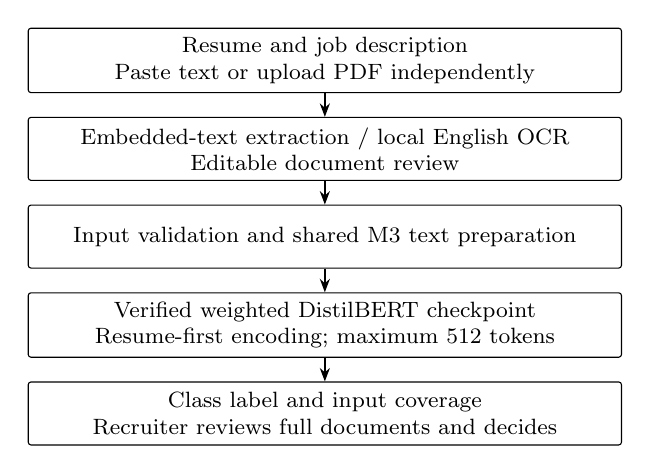
\begin{tikzpicture}[node distance=3mm,box/.style={draw,rounded corners=1pt,align=center,text width=7.3cm,minimum height=8mm,font=\footnotesize},link/.style={-{Stealth[length=1.7mm]},semithick}]
\node[box] (input) {Resume and job description\\Paste text or upload PDF independently};
\node[box,below=of input] (pdf) {Embedded-text extraction / local English OCR\\Editable document review};
\node[box,below=of pdf] (validate) {Input validation and shared M3 text preparation};
\node[box,below=of validate] (model) {Verified weighted DistilBERT checkpoint\\Resume-first encoding; maximum 512 tokens};
\node[box,below=of model] (result) {Class label and input coverage\\Recruiter reviews full documents and decides};
\draw[link] (input)--(pdf);\draw[link] (pdf)--(validate);\draw[link] (validate)--(model);\draw[link] (model)--(result);
\end{tikzpicture}
\caption{Prototype workflow. Pasted text bypasses PDF extraction. Document extraction and classification are separate stages.}
\label{fig:architecture}
\end{figure}

\subsection{PDF Extraction and OCR}
PDFium extracts embedded text. Pages with fewer than 30 alphanumeric characters or excessive replacement characters use Tesseract 5 English OCR; users can also force OCR on every page. Tesseract runs its pretrained LSTM engine with automatic page segmentation \cite{tesseract}. The project integrates this model; it does not train a new OCR model or measure OCR character accuracy.

The reader accepts at most 10~MB and ten pages per document, with a 50,000-character text bound. Page render dimensions are capped at a 2,200-pixel maximum edge. OCR has a 12-second page limit, the worker checks a 45-second document budget, and its parent imposes a 60-second deadline. One extraction worker is admitted per application process. These controls bound work but do not establish a hardened sandbox or eliminate memory-exhaustion risk. Complex columns, poor scans, handwriting, and English-language assumptions require user review.

Uploaded bytes are sent to a local worker through standard input; OCR images are likewise passed to a local subprocess. The application does not write document contents to its own files or send them to an external OCR API. Streamlit session memory and hosting/operating-system handling remain outside any secure-erasure guarantee.

\subsection{Inference and Failure Handling}
The request service validates input before loading the model. It accepts bounded, nonempty strings with alphanumeric content and rejects unsupported control characters. It does not determine whether text is a genuine resume: a short string such as \texttt{abc} can satisfy the input-format checks, and a resulting label would not be meaningful evidence of suitability.

The loader verifies the configured checkpoint against the frozen M4 selection, including its SHA-256 weight hash, three-class mapping, architecture, and input policy. A process-local cache reuses the model, not user documents or predictions. Prediction uses evaluation mode and disabled gradients, with CPU FP32 in the deployed path. A lock serializes access to the shared tokenizer and model call. Errors show safe messages and a request reference rather than raw exceptions. Operational logs contain timing, input lengths, event type, and truncation metadata; document text and predicted labels are excluded.

The deployment downloads only allowed model/tokenizer files from an immutable Hugging Face repository revision when local files are absent. Credentials remain in deployment secrets. Monitoring is manual through platform logs and documented recovery steps; automated alerting and public multi-user capacity validation are not implemented.

\section{Performance and Software Verification}
\subsection{Training and GPU Inference}
The saved MiniLM, original DistilBERT, section-aware, and weighted runs take approximately 4.66, 4.67, 4.60, and 5.12 minutes, respectively, on the recorded T4 runtime. Their reported peak PyTorch allocations are approximately 1.42, 1.95, 1.95, and 1.95~GiB. These are run-specific measurements, not full device memory or a future runtime guarantee.

For the selected saved model, a separate T4 FP16 benchmark uses three warmup batches and 30 timed repeats. Median forward-pass times are 8.804~ms for batch one and 47.271~ms for batch 16. Inputs are already on the GPU; tokenization, transfers, PDF/OCR, browser handling, and output processing are excluded. The original and weighted checkpoints have the same architecture and similar performance; the measurements do not establish a reliable speed advantage.

\subsection{CPU Service Measurements}
Table~\ref{tab:cpu} separates local and hosted CPU service measurements. Both use a repeated synthetic example and 20 sequential warm requests. Service timing covers validation, preparation, token counting, tokenization, inference, response checks, and metadata logging. It excludes imports, network transfer, browser rendering, PDF upload, and OCR.

\begin{table}[t]
\caption{Recorded CPU Service Measurements}
\label{tab:cpu}
\centering\footnotesize
\begin{tabular}{lrr}
\toprule
Measurement & Local macOS & Hosted Linux\\
\midrule
Provision/hash/load (s) & 0.7306 & 0.3438\\
First request after load (ms) & 217.763 & 85.603\\
Warm median (ms) & 29.219 & 63.812\\
Warm P95 (ms) & 40.956 & 147.603\\
RSS baseline (MiB) & 420.27 & 689.16\\
Sampled peak RSS (MiB) & 535.91 & 689.85\\
\bottomrule
\end{tabular}
\end{table}

The local run records eight logical CPUs and four PyTorch threads; the maintainer-supplied hosted report records 16 visible logical CPUs and eight threads. These do not imply dedicated allocation. RSS is sampled every 10~ms and may miss short peaks. The reported load duration does not establish an initial download or complete cold application startup. The hosted evidence confirms selected-weight service inference, but the exact deployed application commit, browser click-to-result timings, and hosted PDF/OCR acceptance remain to be documented.

\subsection{Regression and Artifact Checks}
The latest local verification passes 39 tests with no skips, including CPU model integration, agreement with 30 saved M4 review predictions, real synthetic-PDF OCR, input boundaries, safe failures, stale-result clearing, and PDF worker launch from outside the repository. UI tests use controlled model responses to verify interface behaviour; separate integration tests exercise the selected checkpoint. Agreement on the 30-case private fixture does not establish full validation-set or logit equivalence across versions and hardware.

Saved prediction tables reproduce official-test scores and confusion matrices. Final evaluation artifacts retain their checksum manifest. Notebook executable cells, outputs, execution counts, and metadata are preserved while explanatory Markdown improves navigation. None of these software checks demonstrate improved classifier accuracy.

\section{Limitations, Business Goals, and Future Work}
The original goals include test macro-F1 of at least 0.45, recall of at least 0.35 for every class, processing 1,000 pairs within 30~s on a standard Colab CPU after loading, and a pilot targeting 30\% less screening effort with 70\% recruiter agreement. The selected model does not meet the predictive targets. The CPU service benchmark is not the specified 1,000-pair Colab throughput test, and no recruiter pilot measures time savings or agreement. Business benefits remain proposals rather than observed outcomes.

The principal validity limits are one dataset and random seed, overlapping resumes, unverified label quality and provenance, unresolved data rights, unequal input coverage across approaches, and extensive transformer truncation. Repeated exploration of a single validation set can also favour its particular job distribution. No demographic fairness evaluation is supported by reliable protected-group labels. Selected qualitative cases and synthetic OCR tests do not establish population-level performance.

The application's 512-token context is a substantive functional limit, not a PDF extraction failure. Reading a complete PDF does not mean the classifier sees its entire content. The interface therefore reports shortening and requires human review. Future work should evaluate longer-context or document-chunk approaches under a new, independent protocol, rather than promise that a longer input alone fixes classification. Other priorities are verified labels and data permissions, applicant-disjoint evaluation, repeated-seed uncertainty estimates, qualification-sensitive challenge sets, and a carefully designed user pilot. Calibration or abstention would require implementation and separate validation; neither is claimed here.

\section{Conclusion}
This project delivers a documented NLP workflow from data quality checks through compact-transformer training, improvement experiments, error analysis, and a deployed PDF-capable prototype. Class weighting provides a small validation gain, but the preselected weighted DistilBERT reaches only 0.3563 test macro-F1, below the TF-IDF comparator's 0.4058. Robustness and class-level results show important weaknesses that aggregate scores alone hide. The implementation demonstrates reproducible development and guarded deployment, while its measured predictive limits restrict use to a prototype with human oversight.

\section*{Reproducibility and Availability}
Code, executed notebooks, aggregate reports, and setup instructions are available at \url{https://github.com/nandu-99/resume-job-matcher}. The reported deployment is \url{https://resume-job-matcher-nlp.streamlit.app/}. The core walkthrough uses the M2 preparation/baseline notebooks, M3 shared-split and combined transformer notebook, M4 combined evaluation notebook, and M5 inference, PDF-worker, and service modules. Model files and the source-text review fixture stay outside Git.

The dataset revision is \nolinkurl{08978e21714984bb417547d2c0f9b477f5298163}. The recorded MiniLM revision is \nolinkurl{44acabbec0ef496f6dbc93adadea57f376b7c0ec}; the DistilBERT revision is \nolinkurl{12040accade4e8a0f71eabdb258fecc2e7e948be}. The selected weights have SHA-256 \nolinkurl{004d162ccc9daa4311ff9edeecb1e860a3638a5d0e0c530f5a929df7a40d4b72}. Exact package versions and arguments accompany the experiments. Training records Python 3.13.16 and Transformers 5.24.0; the CPU runtime uses PyTorch 2.10.0 and Transformers 5.3.0, with hosted Linux using the CPU PyTorch build. These environments are distinct and should not be installed over one another during reproduction.

\begin{thebibliography}{10}
\bibitem{siamese} S. Maheshwary and H. Misra, ``Matching resumes to jobs via deep Siamese network,'' in \emph{Companion Proc. Web Conf.}, 2018, pp. 87--88, doi: \href{https://doi.org/10.1145/3184558.3186942}{10.1145/3184558.3186942}.
\bibitem{consultant} D. Lavi, V. Medentsiy, and D. Graus, ``conSultantBERT: Fine-tuned Siamese Sentence-BERT for matching jobs and job seekers,'' \emph{RecSys in HR}, 2021. [Online]. Available: \url{https://arxiv.org/abs/2109.06501}
\bibitem{confit} X. Yu, J. Zhang, and Z. Yu, ``ConFit: Improving resume-job matching using data augmentation and contrastive learning,'' in \emph{Proc. ACM Conf. Recommender Systems}, 2024, pp. 601--611, doi: \href{https://doi.org/10.1145/3640457.3688108}{10.1145/3640457.3688108}.
\bibitem{confit2} X. Yu, R. Xu, C. Xue, J. Zhang, X. Ma, and Z. Yu, ``ConFit v2: Improving resume-job matching using hypothetical resume embedding and runner-up hard-negative mining,'' in \emph{Findings of ACL}, 2025, pp. 12775--12790, doi: \href{https://doi.org/10.18653/v1/2025.findings-acl.661}{10.18653/v1/2025.findings-acl.661}.
% Publisher metadata accessed 26 November 2026 lists Jiaying Jin as author.
\bibitem{calibrated} J. Jin, ``Calibrated resume-job matching for trustworthy LLM-assisted recruiter screening: Pairwise matching, probability calibration, and selective refusal on two public recruitment datasets,'' \emph{J. Technology Informatics and Engineering}, vol. 4, no. 3, 2025, doi: \href{https://doi.org/10.51903/jtie.v4i3.529}{10.51903/jtie.v4i3.529}.
\bibitem{distilbert} V. Sanh, L. Debut, J. Chaumond, and T. Wolf, ``DistilBERT, a distilled version of BERT: Smaller, faster, cheaper and lighter,'' arXiv:1910.01108, 2019. [Online]. Available: \url{https://arxiv.org/abs/1910.01108}
\bibitem{minilm} W. Wang, F. Wei, L. Dong, H. Bao, N. Yang, and M. Zhou, ``MiniLM: Deep self-attention distillation for task-agnostic compression of pre-trained transformers,'' arXiv:2002.10957, 2020. [Online]. Available: \url{https://arxiv.org/abs/2002.10957}
\bibitem{dataset} cnamuangtoun, ``resume-job-description-fit,'' Hugging Face Datasets, recorded revision 08978e2. [Online]. Available: \url{https://huggingface.co/datasets/cnamuangtoun/resume-job-description-fit}
\bibitem{tesseract} Tesseract OCR contributors, ``Command-line usage,'' \emph{Tesseract Documentation}. Accessed: Nov. 26, 2026. [Online]. Available: \url{https://tesseract-ocr.github.io/tessdoc/Command-Line-Usage.html}
\end{thebibliography}
\end{document}
